\documentclass[tikz,border=0pt]{standalone}
\usepackage{pgfplots}
\usepackage{xcolor}
\usetikzlibrary{arrows}
\usetikzlibrary{arrows.meta}

% original colors
\definecolor{color1}{RGB}{166,118,29}
\definecolor{color2}{RGB}{217,95,2}
\definecolor{color3}{RGB}{231,41,138}
\definecolor{color4}{RGB}{117,112,179}
\definecolor{color5}{RGB}{27,158,119}
\definecolor{color6}{RGB}{102,166,30}
\definecolor{color7}{RGB}{230,171,2}

\begin{document}
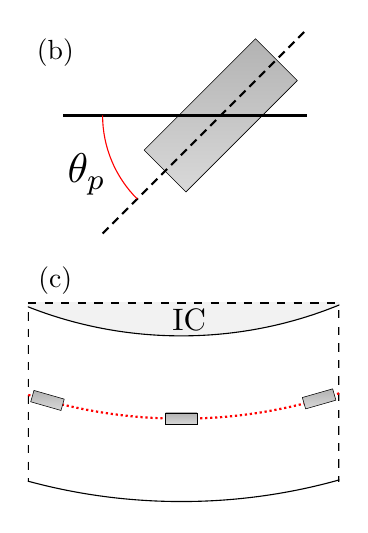
\begin{tikzpicture}
  [
    rec0/.style={shade,
                rectangle,
                minimum width=4mm,
                minimum height=1.5mm,
                inner sep=0pt,
                outer sep=0pt,
                top color=gray!60!white,
                bottom color=gray!30!white,
                draw=black, 
                very thin},
    rec16/.style={shade,
                rectangle,
                rotate=16,
                minimum width=4mm,
                minimum height=1.5mm,
                inner sep=0pt,
                outer sep=0pt,
                top color=gray!60!white,
                bottom color=gray!30!white,
                draw=black, 
                very thin},
    rec16r/.style={shade,
                rectangle,
                rotate=-16,
                minimum width=4mm,
                minimum height=1.5mm,
                inner sep=0pt,
                outer sep=0pt,
                top color=gray!60!white,
                bottom color=gray!30!white,
                draw=black, 
                very thin},
    rec45/.style={shade,
                rectangle,
                rotate=45,
                minimum width=20mm,
                minimum height=7.5mm,
                inner sep=0pt,
                outer sep=0pt,
                top color=gray!60!white,
                bottom color=gray!30!white,
                draw=black, 
                very thin}
  ]
 \begin{scope}[
     scale=4,
     every node/.append style={transform shape},
    ]
    \clip (-0.487, -1.220) rectangle (0.502, -1.86);

    % Outer cylinder and water inside
    \draw[color=black, fill=white, thin] (0, 0) circle (1.851);

    % inner cylinder
    \draw[color=black, fill=gray!10, thin] (0, 0) circle (1.325);

    \draw[color=black, dashed, thick] (-0.487, -1.25) -- (-0.487, -1.79);
    \draw[color=black, dashed, thick] (0.502, -1.243) -- (0.502, -1.79);
    \draw[color=black, dashed, thick] (-0.487, -1.220) -- (0.502, -1.220);
    \node at (0.025, -1.275) {\scalebox{0.28}{IC}};

    % dashed center line
    \draw[color=red, thick, densely dotted] (0, 0) circle (1.588);

 \end{scope}

    % plot fiberes
    \path (0, -6.352) coordinate[rec0];  
    \path (-1.70, -6.12) coordinate[rec16r];  
    \path (1.75, -6.10) coordinate[rec16];  

% big fiber representation
 \begin{scope}[
     yshift=10mm,
     xshift=5mm
    ]
    \path (0, -3.50) coordinate[rec45];  
    \draw[color=black, densely dashed, thick] (-1.5, -5) -- (1.10, -2.4);
    \draw[color=black, thick] (-2, -3.5) -- (1.10, -3.5);
    \draw[color=red] (-1.5, -3.5) arc (180:225:15mm);
    \node at (-1.70, -4.25) {\scalebox{1.5}{$\theta_p$}};
    
\end{scope}

\node at (-1.6, -1.70) {(b)};
\node at (-1.6, -4.60) {(c)};

\end{tikzpicture} 
\end{document}
